\documentclass[12pt]{article}
\usepackage{graphicx} % Required for inserting images
\usepackage{hyperref}
\usepackage{makecell}
\usepackage{makeidx}
\usepackage{eurosym}
\usepackage{amsmath}
\usepackage{fancyhdr}
\usepackage{booktabs} % Per linee orizzontali migliori
\newcommand{\firstPage}{
    \thispagestyle{empty}
    \begin{figure}
    \centering
    
\includegraphics[scale=0.7]{Swellfish_logo.png}
    \end{figure}
    \author{
        \date{}
        \href{mailto://swellfish14@gmail.com}{swellfish14@gmail.com} \\
    } 
}
\usepackage{hyperref}
\usepackage{array}
\usepackage{tabularx}
\usepackage{adjustbox}

\newcounter{verscount}
\setcounter{verscount}{0}
\newcommand{\addversione}[5]{
	\ifdefined\setversione
		\setversione{#1}
	\else\fi
	\stepcounter{verscount}
	\expandafter\newcommand%
		\csname ver\theverscount \endcsname{#1&#2&#3&#4&#5}
}

\newcommand{\listversioni}{
	\ifnum\value{verscount}>1
		\csname ver\theverscount \endcsname
		\addtocounter{verscount}{-1}
		\\\hline
		\listversioni
	\else
		\csname ver\theverscount \endcsname\\\hline
	\fi
}

\newcommand{\makeversioni}{
	\begin{center}
		\begin{tabularx}{\textwidth}{|c|c|X|X|X|}
		\hline
		\textbf{Versione} & \textbf{Data} & \textbf{Redattore} & \textbf{Verificatore} & \textbf{Descrizione} \\
		\hline
		\listversioni
		\end{tabularx}
	\end{center}
	\clearpage
}

\fancypagestyle{genericDocstyle}{
	\pagestyle{fancy}
	\lhead{
\includegraphics[width=1cm]{Swellfish_logo.png}}
	\rhead{Norme di progetto}
}

%\hypersetup{colorlinks=true,urlcolor=blue}

%\newcommand{\tableContent}{

	%{
		%\hypersetup{linkcolor=black}
		%\tableofcontents
	%}
%}
\begin{document}

\graphicspath{ {../templates/img/} {./img}}

\title{Piano di qualifica}

\firstPage

\sethdr{Piano di qualifica}


\maketitle

\begin{center}
	\begin{tabular}{r | l}
		\multicolumn{2}{c}{\textit{Informazioni}}                          \\
		\hline

		\textit{Redattori}    &
		[Davide Porporati, Claudio Giaretta, Francesco Naletto]\makecell{} \\

		\textit{Revisori}     &
		[Jude Vensil Braceros]\makecell{}                                  \\
		\textit{Responsabili} &
		[Andrea Veronese]\makecell{}                                       \\
		\textit{Uso}          &
		[Esterno]\makecell{}                                               \\
	\end{tabular}
\end{center}

\begin{center}
	\textbf{Descrizione}\\
	File contenente il piano di qualifica. Contiene le metriche e i criteri di accettazione dei prodotti.
\end{center}

\pagebreak
\addversione{0.0.1}{25/04/2023}{Andrea Veronese}{Davide Porporati}{Creata struttura di base del documento}
\addversione{0.0.2}{27/04/2023}{Davide Porporati, Elena Marchioro, Francesco Naletto}{Jude Vensil Braceros}{Modificata la struttura del documento}
\addversione{0.1.0}{25/05/2023}{Claudio Giaretta, Francesco Naletto}{Francesco Naletto}{Stesura introduzione, qualità di processo e qualità di prodotto}
\addversione{0.1.1}{13/07/2023}{Claudio Giaretta}{Francesco Naletto}{Aggiornamento dei grafici e aggiunta delle ultime considerazioni del gruppo}
\addversione{1.0.0}{18/07/2023}{Andrea Veronese}{Claudio Giaretta, Davide Porporati}{Aggiornato a versione 1.0.0}
\addversione{1.0.1}{07/06/2023}{Claudio Giaretta}{Andrea Veronese, Davide Porporati}{Creata struttura specifiche di test e aggiunti test di sistema}
\addversione{1.0.2}{07/08/2023}{Andrea Veronese}{Claudio Giaretta, Davide Porporati}{Aggiunte metriche da usare nei test di verifica}
\addversione{1.0.3}{12/09/2023}{Francesco Naletto}{Davide Porporati}{Aggiunta sezione test di unità}
\addversione{1.0.4}{14/09/2023}{Claudio Giaretta}{Francesco Naletto}{Aggiornato Valutazione delle metriche}
\makeversioni
\pagebreak

\tableofcontents
\pagebreak

\printindex



\section{Introduzione}
\subsection{Scopo del documento}
Questo documento ha lo scopo di definire le strategia di validazione e verifica addottate per garantire la qualità del prodotto.
Per raggiungere questo obbiettivo viene applicato un sistema di verifica continua sui processi e sulle attività del gruppo, questo permette di ottenere un miglioramento continuo.
Il documento non ha una funzione descrittiva, la definizione delle metriche indicate all'interno di questo documento, è presente nel documento "norme\_di\_progetto".
\section{Qualità di processo}

\subsection{Processi primari}

\subsubsection{Fornitura}
\textbf{Metriche:}
\begin{itemize}
	\item MPC01: Actual Cost (AV)
	      \begin{itemize}
		      \item \textbf{Calcolo della metrica}: Somma dei costi tracciati dal gruppo
		      \item \textbf{Valore ottimale}: $\le BAC$
		      \item \textbf{Valore accettabile}: $\le BAC$
	      \end{itemize}
	\item MPC02: Planned Value (PV)
	      \begin{itemize}
		      \item \textbf{Calcolo della metrica}: Percentuale di completamento del progetto pianificata * BAC
		      \item \textbf{Valore ottimale}: $\le BAC$
		      \item \textbf{Valore accettabile}: $\le BAC$
	      \end{itemize}
	\item MPC03: Earned Value (EV)
	      \begin{itemize}
		      \item \textbf{Calcolo della metrica}: Percentuale dell'effettivo stato di completamento del progetto * BAC
		      \item \textbf{Valore ottimale}: $\ge 0$
		      \item \textbf{Valore accettabile}: $\le BAC$
	      \end{itemize}
	\item MPC04: Cost Variance (CV)
	      \begin{itemize}
		      \item \textbf{Calcolo della metrica}:  EV - AC
		      \item \textbf{Valore ottimale}: $\ge 0\%$
		      \item \textbf{Valore accettabile}: $\ge -12\%$
	      \end{itemize}
	\item MPC05: Schedule Variance (SV)
	      \begin{itemize}
		      \item \textbf{Calcolo della metrica}:  EV - PV
		      \item \textbf{Valore ottimale}: $\ge 0\%$
		      \item \textbf{Valore accettabile}: $\ge -12\%$
	      \end{itemize}

	\item MPC06: Cost Performance Index (CPI)
	      \begin{itemize}
		      \item \textbf{Calcolo della metrica}:  EV / AC
		      \item \textbf{Valore ottimale}: $\ge 1$
		      \item \textbf{Valore accettabile}: $\ge 0,9$
	      \end{itemize}

	\item MPC07: Estimated At Completition (EAC)
	      \begin{itemize}
		      \item \textbf{Calcolo della metrica}:  BAC / CPI
		      \item \textbf{Valore ottimale}: = BAC
		      \item \textbf{Valore accettabile}: $\ge BAC - 3\% ; \le BAC + 3\% $
	      \end{itemize}
	\item MPC08: Estimate To Completition (ETC)
	      \begin{itemize}
		      \item \textbf{Calcolo della metrica}:  (BAC - EV) / CPI
		      \item \textbf{Valore ottimale}: $\ge 0\%$
		      \item \textbf{Valore accettabile}: $\le EAC$
	      \end{itemize}
\end{itemize}

\subsection{Processi di supporto}
\subsubsection{Documentazione}
\textbf{Metriche:}
\begin{itemize}
	\item MPC09: Indice di Gulpease
	      \begin{itemize}
		      \item \textbf{Calcolo della metrica}:  89 + $\frac{300*(F) - 10 * (L)}{(P)}$
		            \begin{itemize}
			            \item \textbf{L} = Numero di lettere nel testo
			            \item \textbf{P} = Numero di parole nel testo
			            \item \textbf{F} = Numero di frasi nel testo
		            \end{itemize}
		      \item \textbf{Valore ottimale}: 100 \%
		      \item \textbf{Valore accettabile}: $\ge 60\%$
	      \end{itemize}
\end{itemize}
\begin{itemize}
	\item MPC10: Errori ortografici
	      \begin{itemize}
		      \item \textbf{Calcolo della metrica}: numero errori ortografici presenti nel testo
		      \item \textbf{Valore ottimale}: 0
		      \item \textbf{Valore accettabile}: 0
	      \end{itemize}
\end{itemize}

\subsubsection{Verifica}

\textbf{Metriche:}
\begin{itemize}
	\item MPC11: Statement Coverage. \\
	      La metrica si basa sullo statement coverage.
	      Indica la percentuale di statement eseguiti almeno una volta dall'insieme dei testi di unità.\\
	      I valori sono forniti dalla suite di testing Jest.

	      \begin{center}
		      \begin{tabularx}{\textwidth}{|X|X|X|}
			      \hline
			      \textbf{Prodotto} & \textbf{Valore accettabile } & \textbf{Valore ottimale } \\
			      \hline
			      Software          & $>$ 80\%                     & $>$ 95\%                  \\
			      \hline
		      \end{tabularx}\\[8pt]
		      \mbox{}\\
	      \end{center}

	\item MPC12: Branch Coverage \\
	      La metrica si basa sul branch coverage. Indica la percentuale di branch che vengono testati almeno una volta, con esito positivo. \\
	      Valori fonriti dal report di Jest.

	      \begin{center}
		      \begin{tabularx}{\textwidth}{|X|X|X|}
			      \hline
			      \textbf{Prodotto} & \textbf{Valore accettabile } & \textbf{Valore ottimale } \\
			      \hline
			      Software          & $>$ 75\%                     & $>$ 95\%                  \\
			      \hline
		      \end{tabularx}\\[8pt]
		      \mbox{}\\
	      \end{center}

	\item MPC13: Code Coverage \\
	      La metrica si basa sul code coverage. Indica la percentuale di codice eseguito nella fase di testing. \\
	      Valori fonriti dal report di Jest.

	      \begin{center}
		      \begin{tabularx}{\textwidth}{|X|X|X|}
			      \hline
			      \textbf{Prodotto} & \textbf{Valore accettabile } & \textbf{Valore ottimale } \\
			      \hline
			      Software          & $>$ 80\%                     & $>$ 95\%                  \\
			      \hline
		      \end{tabularx}\\[8pt]
		      \mbox{}\\
	      \end{center}

	\item MPC14: Condition Coverage \\
	      La metrica si basa sul condition coverage. Indica la percentuale di branch che risultano almeno una volta true e almeno una volta false nell'esecuzione di un test dedicato. \\
	      Valori fonriti dal report di Jest.

	      \begin{center}
		      \begin{tabularx}{\textwidth}{|X|X|X|}
			      \hline
			      \textbf{Prodotto} & \textbf{Valore accettabile } & \textbf{Valore ottimale } \\
			      \hline
			      Software          & $>$ 70\%                     & $>$ 80\%                  \\
			      \hline
		      \end{tabularx}\\[8pt]
		      \mbox{}\\
	      \end{center}

\end{itemize}


\subsection{Processi organizzativi}

\section{Qualità di prodotto}
\subsection{Introduzione}
Per assicurare la qualità del prodotto, abbiamo adottato lo standard ISO/IEC 9126 come punto di riferimento. In questa sezione, forniamo i valori ottimali e accettabili per le metriche selezionate dal gruppo SWEllFish.



\subsection{Affidabilità}
\textbf{Metriche}:
\begin{itemize}
	\item MPD01: Percentuale di difetti del prodotto.
	      \begin{itemize}
		      \item Valore ottimale: 80\%.
		      \item Valore accettabile: 60\%.
		      \item Note: I valori possono essere modificati.
	      \end{itemize}
\end{itemize}


\subsection{Efficienza}
\textbf{Metriche}:
\begin{itemize}
	\item MPD02: Tempo medio di risposta.
	      \begin{itemize}
		      \item Metrica di misurazione: Secondi.
		      \item Valore ottimale: 5 secondi.
		      \item Valore accettabile: 7 secondi.
	      \end{itemize}
\end{itemize}

\subsection{Funzionalità}
\textbf{Metriche}:
\begin{itemize}
	\item MPD03: Percentuale di copertura dei requisiti.
	      \begin{itemize}
		      \item Valore ottimale: 100\% dei requisiti obbligatori e 80\% dei requisiti opzionali.
		      \item Valore accettabile: 100\% dei requisiti obbligatori.
	      \end{itemize}
\end{itemize}

\subsection{Manutenibilità}
\textbf{Metriche}:
\begin{itemize}
	\item MPD04: Percentuale di comprensibilità del codice.
	      \begin{itemize}
		      \item Valore ottimale: 85\% - 100\%.
		      \item Valore accettabile: 65\%.
	      \end{itemize}
\end{itemize}


\subsection{Portabilità}
\textbf{Metriche}:
\begin{itemize}
	\item MPD05: Percentuale di compatibilità del prodotto.
	      \begin{itemize}
		      \item Valore ottimale: 85\% - 100\%.
		      \item Valore accettabile: 60\%.
	      \end{itemize}
\end{itemize}


\subsection{Usabilità}
\textbf{Metriche:}
\begin{itemize}
	\item MPD06: Numero di errori compiuti dagli utenti durante l'utilizzo del prodotto.
	      \begin{itemize}
		      \item Valore ottimale: Inferiore a 1 errore per utente.
		      \item Valore accettabile: Inferiore a 2 errori per utente.
	      \end{itemize}
\end{itemize}


\section{Specifica di test}
\subsection{Test di accettazione}
I test di accettazione sono essenziali per dimostrare la conformità del prodotto ai requisiti minimi concordati con il proponente. Questa fase comprende i test di sistema che vengono condotti durante il collaudo finale, coinvolgendo sia i membri del team di sviluppo che i rappresentanti dell'azienda proponente. L'intero processo è attentamente sorvegliato dal nostro gruppo.
\subsection{Test di sistema}
\begin{xltabular}{\linewidth}{|>{\hsize=0.6\hsize}X|>{\hsize=2.3\hsize}X|>{\hsize=0.7\hsize}X|>{\hsize=0.4\hsize}X|}

	\hline
	\textbf{ID Test} & \textbf{Descrizione} & \textbf{Requisito} & \textbf{Stato} \\
	\hline
	\endfirsthead
	\hline
	\textbf{ID Test} & \textbf{Descrizione} & \textbf{Requisito} & \textbf{Stato} \\
	\hline
	\endhead
	\hline
	\endfoot
	TS1	 & Verificare che l'utente riesca ad effettuare correttamente l'accesso a sistema	&	RF1	&	NI	\\
	\hline
	TS2	 & Verificare che l'utente visualizzi correttamente lo stato del sistema	&	RF2	&	NI	\\
	\hline
	TS3	 & Verificare che l'utente sia in grado di cambiare la luminosità correttamente	&	RF3	&	NI	\\
	\hline
	TS4	 & Verificare che il sistema visualizzi correttamente il messaggio di errore nel caso in cui l'aumento della luminosità non fosse andato a buon fine 	&	RF4	&	NI	\\
	\hline
	TS5	& Verificare che l'utente possa visualizzare correttamente la lista delle aree illuminate	&	RF5 	&	NI	\\
	\hline
	TS6	& Verificare che l'utente possa vedere correttamente l'elenco delle zone	&	RF6	&	NI	\\
	\hline
	TS7	 & Verificare che l'utente possa selezionare le zone correttamente	&	RF7	&	NI	\\
	\hline
	TS8	 & Verificare che l'utente possa diminuire la luminosità di una zona correttamente	&	RF8	&	NI	\\
	\hline
	TS9	 & Verificare che l'utente possa accedere correttamente alla dashboard	&	RF10	&	NI	\\
	\hline
	TS10	 & Verificare che il sistema visualizzi correttamente il messaggio di errore nel caso la diminuzione della luminosità non fosse andata a buon fine 	&	RF11	&	NI	\\
	\hline
	TS11	 & Verificare che l'utente possa diminuire la luminosità correttamente	&	RF12	&	NI	\\
	\hline
	TS12	 & Verificare che l'utente possa inserire una nuova area illuminata correttamente	&	RF13	&	NI	\\
	\hline
	TS13	 & Verificare che l'utente possa rimuovere un area di illuminazione correttamente	&	RF14	&	NI	\\
	\hline
	TS14	 & Verificare che l'utente possa accedere alla lista delle zone gestite correttamente	&	RF15	&	NI	\\
	\hline
	TS15	 & Verificare che l'utente possa modificare le informazioni di un area illuminata	&	RF16	&	NI	\\
	\hline
	TS16	 & Verificare che il sisteam mostri correttamente il messaggio di notifica una volta fatta la modifica all'area illuminata 	&	RF17	&	NI	\\
	\hline
	TS17	 & Verificare che l'utente possa inserire correttamente un sensore in un area illuminata	&	RF18	&	NI	\\
	\hline
	TS18	 & Verificare che l'utente possa accedere correttamente all'area illuminata	&	RF19	&	NI	\\
	\hline
	TS19	 & Verificare che l'utente possa rimuovere un sensore dall'area illuminata	&	RF20	&	NI	\\
	\hline
	TS20	 & Verificare che l'utente possa fare il logout dal sistema correttamente	&	RF21	&	NI	\\
	\hline
	TS21	 & Verificare che l'utente possa inserire un impianto nell'elenco dei guasti correttamente	&	RF22	&	NI	\\
	\hline
	TS22	 & Verificare che l'utente possa rimuovere un impianto dall'elenco dei guasti correttamente	&	RF23	&	NI	\\
	\hline
	TS23	 & Verificare che l'utente possa visualizzare i dettagli di una zona correttamente	&	RF24	&	NI	\\
	\hline
	TS24	 & Verificare che l'utente possa selezionare un lampione correttamente	&	RF25	&	NI	\\
	\hline
	TS25	 & Verificare che l'utente possa visualizzare i dettagli di un lampione correttamente	&	RF26	&	NI	\\
	\hline
	TS26	 & Verificare che l'utente possa inserire un nuovo lampione all'interno di un'area illuminata correttamente	&	RF27	&	NI	\\
	\hline
	TS27	 & Verificare che l'utente possa rimuovere un lampione all'interno di un'area illuminata correttamente	&	RF28	&	NI	\\
	\hline
	TS28	 & Verificare che l'utente possa visualizzare l'elenco delle aree illuminate con dei malfunzionamenti correttamente	&	RF29	&	NI	\\
	\hline
	TS29	 & Verificare che l'amministratore possa poter aprire una nuova segnalazione di un guasto tramite un ticket	&	RF30	&	NI	\\
	\hline
	TS30	 & Verificare che l'amministratire possa poter chiudere il ticket dopo aver fatto la dovuta manutenzione correttamente	&	RF31	&	NI	\\
	\hline
	TS31	 & Verificare che il manutentore possa visualizzare i dettagli aggiuntivi di un guasto forniti dal ticket correttamente	&	RF32	&	NI	\\
	\hline
	TS32	 & Verificare che l'utente non amministratore possa riceve le credenziali di amministratore da un superamministratore	&	RF33	&	NI	\\
	\hline
	TS33	 & Verificare che l'utente possa consultare il manuale Lumos Minima	&	RF34	&	NI	\\
	\hline
	TS34	 & Verificare che le nuove aree illuminate appena inserite abbiano un setup standard	&	RF35	&	NI	\\

\end{xltabular}

\subsection{Test di integrazione}
\footnotesize
\begin{xltabular}{\linewidth}{|>{\hsize=0.2\hsize}X|X|>{\hsize=0.1\hsize}X|}

	\hline
	\textbf{ID Test} & \textbf{Descrizione} & \textbf{Stato} \\
	\hline
	\endfirsthead
	\hline
	\textbf{ID Test} & \textbf{Descrizione}  & \textbf{Stato} \\
	\hline
	\endhead
	\hline
	\endfoot
	TI1 & Verificare che il collegamento con backend avvenga correttamente. & S \\ \hline
	TI2 & Verificare che il collegamento con simulatori avvenga correttamente. & S \\ \hline


\end{xltabular}

\subsection{Test di unità}
\subsubsection{Test di unità - Frontend}
\footnotesize
\begin{xltabular}{\linewidth}{|>{\hsize=0.2\hsize}X|X|>{\hsize=0.1\hsize}X|}

	\hline
	\textbf{ID Test} & \textbf{Descrizione} & \textbf{Stato} \\
	\hline
	\endfirsthead
	\hline
	\textbf{ID Test} & \textbf{Descrizione}  & \textbf{Stato} \\
	\hline
	\endhead
	\hline
	\endfoot
	TU01 & Verifica che il componente AggiungiAreaView venga renderizzato correttamente & S \\ \hline
	TU02 & Verifica che venga renderizzato un messaggio di errore quando il valore di submitIsError è true & S \\ \hline
	TU03 & Verifica che vengano cancellati gli errori correttamente & S \\ \hline
	TU04 & Verifica che il componente AggiungiGuastoView venga renderizzato correttamente & S \\ \hline
	TU05 & Verifica che venga renderizzato un messaggio di errore quando il valore di submitIsError è true & S \\ \hline
	TU06 & Verifica che venga renderizzato correttamente se areaDetails non è definita & S \\ \hline
	TU07 & Verifica che il componente AggiungiLampioneView venga renderizzato correttamente & S \\ \hline
	TU08 & Verifica che venga renderizzato un messaggio di errore quando il valore di submitIsError è true & S \\ \hline
	TU09 & Verifica che il componente AggiungiSensoreView venga renderizzato correttamente & S \\ \hline
	TU10 & Verifica gestione dei submit con errore & S \\ \hline
	TU11 & Verifica gestione cambiamenti agli input del form & S \\ \hline
	TU12 & Verifica chiamata a clearError onFormFocus & S \\ \hline
	TU13 & Verifica se il componente AreaDetailsView viene renderizzato correttamente quando il caricamento è in corso. Il test cerca la presenza del testo "Loading..." nella vista. & S \\ \hline
	TU14 & Verifica se il componente AreaDetailsView viene renderizzato correttamente quando non ci sono errori. Il test cerca la presenza del testo "Dettagli area" nella vista. & S \\ \hline
	TU15 & Verifica se il pulsante "Accendi Lampioni Area" reagisce correttamente al click, ossia se chiama la funzione accendiLampioniArea del ViewModel. & S \\ \hline
	TU16 & Verifica se il pulsante "Aumenta Luminosità" reagisce correttamente al click, ossia se chiama la funzione aumentaLuminosità del ViewModel. & S \\ \hline
	TU17 & Verifica se il pulsante "Diminuisci Luminosità" reagisce correttamente al click, ossia se chiama la funzione diminuisciLuminosità del ViewModel. & S \\ \hline
	TU18 & Verifica se il pulsante "Spegni Lampioni Area" reagisce correttamente al click, ossia se chiama la funzione spegniLampioniArea del ViewModel. & S \\ \hline
	TU19 & Verifica se il pulsante "Cambia Modalità" reagisce correttamente al click, ossia se chiama la funzione cambiaModalità del ViewModel. & S \\ \hline
	TU20 & Verifica se il pulsante "Elimina Area" reagisce correttamente al click, ossia se chiama la funzione eliminaArea del ViewModel. & S \\ \hline
	TU21 & Verifica se il componente AreaDetailsView gestisce correttamente lo stato di errore, inclusa la visualizzazione del messaggio di errore. & S \\ \hline
	TU22 & Verifica se il componente AreaDetailsView mostra correttamente lo stato "Acceso" quando il ViewModel lo specifica. & S \\ \hline
	TU23 & Verifica se il componente AreaDetailsView mostra correttamente la luminosità in modalità automatica quando il ViewModel lo specifica. & S \\ \hline
	TU24 & Verifica come il componente AreaDetailsView gestisce gli errori di submit quando submitHasError è true. & S \\ \hline
	TU25 & Verifica come il componente AreaDetailsView gestisce il rendering quando i dati sono undefined. & S \\ \hline
	TU26 & viene verificato se il componente AreeView viene renderizzato correttamente. & S \\ \hline
	TU27 & viene verificato se il componente AreeView gestisce correttamente lo stato di caricamento quando isLoading è impostato su true. & S \\ \hline
	TU28 & viene verificato se il componente GuastoDetailsView viene renderizzato correttamente. & S \\ \hline
	TU29 & verifica se il messaggio di caricamento "Loading..." è presente nella vista. & S \\ \hline
	TU30 & verifica se un messaggio di errore è presente nella vista. & S \\ \hline
	TU31 & verifica se la funzione chiudiGuasto del ViewModel è stata chiamata correttamente. & S \\ \hline
	TU32 & verifica che il componente non venga renderizzato quando stato è uguale a "1". In altre parole, si verifica che il componente non sia visibile nella vista. & S \\ \hline
	TU33 & verifica che il componente venga renderizzato correttamente quando stato è diverso da "1". In questo caso, si verifica la presenza del testo "Impostazioni Guasto" nella vista. & S \\ \hline
	TU34 & verifica che il componente sia ancora in grado di renderizzare correttamente anche quando i dati di guastoDetails sono undefined. & S \\ \hline
	TU35 & verificato se il componente HomeView viene renderizzato correttamente. & S \\ \hline
	TU36 & verifica se i messaggi di caricamento "Loading..." sono presenti nella vista. & S \\ \hline
	TU37 & viene verificato se il pulsante "Logout" è presente nella vista. Successivamente simula un clic su questo pulsante e verifica se la funzione logout del ViewModel è stata chiamata correttamente & S \\ \hline
	TU38 & verifica se gli elementi dei guasti sono stati renderizzati correttamente, confrontando i dati dei guasti presenti nel mock ViewModel con il testo previsto nella vista. & S \\ \hline
	TU39 & verificato se il componente ListaGuastiView viene renderizzato correttamente. & S \\ \hline
	TU40 &  verifica se il messaggio di caricamento "Loading..." è presente nella vista. & S \\ \hline
	TU41 & verifica se il componente viene ancora renderizzato correttamente senza errori quando i dati sono mancanti. & S \\ \hline
	TU42 & viene verificato se il componente ListaLampioniView viene renderizzato correttamente. & S \\ \hline
	TU43 & verifica se il messaggio di caricamento "Loading..." è presente nella vista. & S \\ \hline
	TU44 & erifica se i dettagli dei lampioni sono visualizzati correttamente, compresi ID, IP, stato e tipo di interazione. & S \\ \hline
	TU45 & Verifica se la funzione accendiLampione viene chiamata con l'ID corretto del lampione. & S \\ \hline
	TU46 & verifica se il componente viene ancora renderizzato correttamente senza errori quando i dati sono mancanti. & S \\ \hline
	TU47 & verifica se il componente viene renderizzato correttamente, inclusi i dettagli dei sensori (ID, IP, tipo di interazione, polling time e raggio di azione). & S \\ \hline
	TU48 & verifica se il messaggio di caricamento "Loading..." è presente nella vista. & S \\ \hline
	TU49 & verifica se il componente viene renderizzato correttamente e se il testo "Login" è presente nell'output. & S \\ \hline
	TU50 & verifica se il componente viene renderizzato correttamente e se i campi di input contengono i valori corrispondenti ai dettagli dell'area forniti dal ViewModel. & S \\ \hline
	TU51 & verifica se la funzione submit del ViewModel (mockViewModel.submit) è stata chiamata con i valori aggiornati del form. Ciò assicura che il form venga sottomesso correttamente con i dati modificati. & S \\ \hline
	TU52 & verifica se tutti i campi di input sono vuoti o nulli quando non ci sono dati dell'area disponibili. Questo copre il caso in cui l'utente voglia creare una nuova area e non ci siano dati preesistenti. & S \\ \hline
	TU53 & verifica se il componente viene renderizzato correttamente e se i campi di input contengono i valori corrispondenti ai dettagli del guasto forniti dal ViewModel. & S \\ \hline
	TU54 & verifica se la funzione submit del ViewModel (mockViewModel.submit) è stata chiamata con i valori aggiornati del form. Ciò assicura che il form venga sottomesso correttamente con i dati modificati. & S \\ \hline
	TU55 & verifica che il componente venga renderizzato correttamente anche quando lo stato del guasto è 1. & S \\ \hline
	TU56 & verifica se tutti i campi di input sono vuoti o nulli quando non ci sono dati del guasto disponibili. Questo copre il caso in cui l'utente voglia creare un nuovo guasto e non ci siano dati preesistenti. & S \\ \hline
	TU57 & verifica se il componente viene renderizzato correttamente e se i campi di input contengono i valori corrispondenti ai dettagli del lampione forniti dal ViewModel. & S \\ \hline
	TU58 & verifica se la funzione modificaLampione del ViewModel (mockViewModel.modificaLampione) è stata chiamata con i valori aggiornati del form. Ciò assicura che il form venga sottomesso correttamente con i dati modificati. & S \\ \hline
	TU59 & verifica se viene visualizzato un messaggio di errore appropriato quando si verifica un errore durante il submit del form. & S \\ \hline
	TU60 & verifica se la funzione eliminaLampione del ViewModel (mockViewModel.eliminaLampione) è stata chiamata quando l'utente fa clic sul pulsante. & S \\ \hline
	TU61 & erifica se tutti i campi di input sono vuoti o nulli quando non ci sono dati del lampione disponibili. Questo copre il caso in cui l'utente voglia creare un nuovo lampione e non ci siano dati preesistenti. & S \\ \hline
	TU62 & verifica se il componente viene renderizzato correttamente e se i campi di input contengono i valori corrispondenti ai dettagli del sensore forniti dal ViewModel. & S \\ \hline
	TU63 &  verifica se la funzione submit del ViewModel (mockViewModel.submit) è stata chiamata con i valori aggiornati del form. Ciò assicura che il form venga sottomesso correttamente con i dati modificati. & S \\ \hline
	TU64 & verifica se viene visualizzato un messaggio di errore appropriato quando si verifica un errore durante il submit del form. & S \\ \hline
	TU65 & verifica se la funzione eliminaSensore del ViewModel (mockViewModel.eliminaSensore) è stata chiamata quando l'utente fa clic sul pulsante. & S \\ \hline
	TU66 & verifica se tutti i campi di input sono vuoti o nulli quando non ci sono dati del sensore disponibili. Questo copre il caso in cui l'utente voglia creare un nuovo sensore e non ci siano dati preesistenti. & S \\ \hline
	TU67 & verifica se la funzione mutateAsync del aggiungiAreaMutation nell'oggetto areeStoreMock è stata chiamata. & S \\ \hline
	TU68 & verificato se la funzione submitIsError restituisce true quando submitError nell'oggetto areeStoreMock è impostato su un valore diverso da una stringa vuota. & S \\ \hline
	TU69 & verifica se la funzione setSubmitError nell'oggetto areeStoreMock è stata chiamata con il messaggio di errore restituito dalla chiamata a mutateAsync. & S \\ \hline
	TU70 & verifica che le proprietà e i metodi del ViewModel restituiscano valori definiti, confermando che il ViewModel sia stato creato correttamente e abbia le proprietà e i metodi attesi. & S \\ \hline
	TU71 & verifica se i metodi del store (mockStore) vengono chiamati correttamente quando vengono invocati i metodi del ViewModel. & S \\ \hline
	TU72 & verifica il comportamento del ViewModel quando si verifica un errore durante il submit. & S \\ \hline
	TU73 & verifica che le proprietà e i metodi del ViewModel restituiscano valori definiti, confermando che il ViewModel sia stato creato correttamente e abbia le proprietà e i metodi attesi. & S \\ \hline
	TU74 & verifica se i metodi del store (mockStore) vengono chiamati correttamente quando vengono invocati i metodi del ViewModel.  & S \\ \hline
	TU75 & verifica il comportamento del ViewModel quando si verifica un errore durante il submit. & S \\ \hline
	TU76 & verifica se la funzione getAreaDetails viene chiamata con l'ID corretto quando viene creato un'istanza di AreaDetailsViewModel. & S \\ \hline
	TU77 & verifica se la funzione isLoading restituisce true quando getAreaDetails restituisce un oggetto con isLoading impostato su true. & S \\ \hline
	TU78 & verifica se la funzione isError restituisce false quando getAreaDetails restituisce un oggetto con isError impostato su false. & S \\ \hline
	TU79 & verifica se la funzione aumentaLuminosità chiama la mutazione aumentaLuminositàMutation quando le condizioni sono soddisfatte. & S \\ \hline
	TU80 & verifica che la funzione aumentaLuminosità non chiami la mutazione aumentaLuminositàMutation quando la luminosità è già al massimo. & S \\ \hline
	TU81 & verifica se la funzione diminuisciLuminosità chiama la mutazione diminuisciLuminositàMutation quando le condizioni sono soddisfatte. & S \\ \hline
	TU82 & verifica che la funzione diminuisciLuminosità non chiami la mutazione diminuisciLuminositàMutation quando la luminosità è già al minimo. & S \\ \hline
	TU83 & verifica se la funzione eliminaArea chiama la mutazione eliminaAreaMutation. & S \\ \hline
	TU84 & verifica se la funzione cambiaModalità chiama la mutazione cambiaModalitaMutation. & S \\ \hline
	TU85 & verifica se la funzione accendiArea chiama la mutazione accendiAreaMutation. & S \\ \hline
	TU86 & verifica se la funzione accendiLampioniArea chiama la mutazione accendiLampioniAreaMutation. & S \\ \hline
	TU87 & verifica se la funzione spegniLampioniArea chiama la mutazione spegniLampioniAreaMutation. & S \\ \hline
	TU88 &  verifica se la funzione aree restituisce un array contenente le aree simulate & S \\ \hline
	TU89 & verifica se la funzione isLoading restituisce false quando areeStoreMock ha isLoading impostato su false. & S \\ \hline
	TU90 & verifica se la funzione aumentaLuminositaCrepuscolo chiama la mutazione accendiAllAreeMutationMock.mutateAsync con gli argomenti previsti. In questo caso, viene verificato che sia chiamato senza argomenti (l'oggetto vuoto \{\}). & S \\ \hline
	TU91 & verifica se la funzione diminuisciLuminositaCrepuscolo chiama la mutazione spegniAllAreeMutationMock.mutateAsync con gli argomenti previsti. In questo caso, viene verificato che sia chiamato senza argomenti (l'oggetto vuoto \{\}). & S \\ \hline
	TU92 & verifica se la funzione getGuastoDetails viene chiamata con l'ID corretto quando viene creato un'istanza di GuastoDetailsViewModel. & S \\ \hline
	TU93 & verifica se la funzione chiudiGuasto chiama la mutazione chiudiGuastoMutation e la funzione navigate con gli argomenti previsti quando è chiamata. Viene simulata una risposta di successo dalla mutazione. & S \\ \hline
	TU94 & verifica se la funzione numeroAree restituisce il numero corretto di aree, che è impostato come 10 nella simulazione areeStoreMock. & S \\ \hline
	TU95 & verifica se la funzione numeroAreeisLoading restituisce false, poiché numeroAree non è in stato di caricamento (isLoading è false). & S \\ \hline
	TU96 & verifica se la funzione areeLimit restituisce correttamente la lista delle aree simulate, che è stata impostata come aree nella simulazione areeStoreMock. & S \\ \hline
	TU97 & verifica se la funzione areeLimitisLoading restituisce true, poiché areeLimit è in stato di caricamento (isLoading è true). & S \\ \hline
	TU98 & verifica se la funzione guastiNumber restituisce il numero corretto di guasti, che è impostato come 5 nella simulazione guastiStoreMock. & S \\ \hline
	TU99 & verifica se la funzione guastiNumberisLoading restituisce false, poiché guastiNumber non è in stato di caricamento (isLoading è false). & S \\ \hline
	TU100 & verifica se la funzione guasti restituisce correttamente la lista dei guasti simulati, che è stata impostata come guasti nella simulazione guastiStoreMock. & S \\ \hline
	TU101 & verifica se la funzione guastiisLoading restituisce false, poiché la lista dei guasti non è in stato di caricamento (isLoading è false). & S \\ \hline
	TU102 & verifica se la funzione lampioniNumber restituisce il numero corretto di lampioni, che è impostato come 3 nella simulazione lampioniStoreMock. & S \\ \hline
	TU103 & verifica se la funzione lampioniisLoading restituisce false, poiché il numero di lampioni non è in stato di caricamento (isLoading è false). & S \\ \hline
	TU104 & verifica se la funzione sensoriNumber restituisce il numero corretto di sensori, che è impostato come 7 nella simulazione sensoriStoreMock. & S \\ \hline
	TU105 & verifica se la funzione sensoriisLoading restituisce false, poiché il numero di sensori non è in stato di caricamento (isLoading è false). & S \\ \hline
	TU106 & verifica se la funzione guastiAperti chiama correttamente getGuastiAperti dallo store dei guasti. & S \\ \hline
	TU107 & verifica se la funzione guastiChiusi restituisce un array vuoto e chiama correttamente getGuastiChiusi dallo store dei guasti.  & S \\ \hline
	TU108 & verifica se la funzione isLoading restituisce false. & S \\ \hline
	TU109 & verifica se la funzione areaDetails chiama correttamente getAreaDetails dallo store delle aree.  & S \\ \hline
	TU110 & verifica se la funzione dettagliLampione chiama correttamente getdettagliLampioni dallo store dei lampioni.  & S \\ \hline
	TU111 & verifica se la funzione listaLampioni chiama correttamente getlistaLampioni dallo store dei lampioni. & S \\ \hline
	TU112 & verifica se la funzione isLoading chiama correttamente getlistaLampioni dallo store dei lampioni.  & S \\ \hline
	TU113 & verifica se la funzione accendiLampione chiama correttamente accendiLampioneMutation.mutateAsync dallo store dei lampioni con gli argomenti corretti. & S \\ \hline
	TU114 & verifica se la funzione spegniLampione chiama correttamente spegniLampioneMutation.mutateAsync dallo store dei lampioni con gli argomenti corretti. & S \\ \hline
	TU115 & verifica se la funzione listaSensori chiama correttamente getlistaSensori dallo store dei sensori.  & S \\ \hline
	TU116 & verifica se la funzione isLoading chiama correttamente getlistaSensori dallo store dei sensori.  & S \\ \hline
	TU117 & verifica se la funzione submit del LoginViewModel funziona correttamente. & S \\ \hline
	TU118 & verifica se il ViewModel restituisce tutti i metodi e le variabili attesi.  & S \\ \hline
	TU119 & verifica se i metodi del negozio (getAreaDetails e modificaAreaMutation.mutateAsync) vengono chiamati correttamente quando i metodi del ViewModel (areaDetails, submit, ecc.) vengono invocati.  & S \\ \hline
	TU120 & verifica se i metodi del negozio (getAreaDetails e modificaAreaMutation.mutateAsync) vengono chiamati correttamente quando i metodi del ViewModel (areaDetails, submit, ecc.) vengono invocati.  & S \\ \hline
	TU121 & erifica se il ViewModel restituisce tutti i metodi e le variabili attesi.  & S \\ \hline
	TU122 & verifica se i metodi del negozio (getGuastoDetails e modificaGuastoMutation.mutateAsync) vengono chiamati correttamente quando i metodi del ViewModel (guastoDetails, submit, ecc.) vengono invocati.  & S \\ \hline
	TU123 & verifica se il ViewModel gestisce correttamente gli errori durante l'invio del modulo. & S \\ \hline
	TU124 & erifica se il ViewModel restituisce tutti i metodi e le variabili attesi.  & S \\ \hline
	TU125 & verifica se i metodi del negozio (getdettagliSensori, modificaSensoreMutation.mutateAsync, eliminaSensoreMutation.mutateAsync) vengono chiamati correttamente quando i metodi del ViewModel (sensoreDetails, submit, eliminaSensore, ecc.) vengono invocati. & S \\ \hline
	TU126 & verifica se il ViewModel gestisce correttamente gli errori durante l'invio del modulo. & S \\ \hline


\end{xltabular}

\subsubsection{Tracciamento test di unità - Frontend}
\begin{scriptsize}
\begin{xltabular}{\linewidth}{|>{\hsize=0.1\hsize}X|X|}

	\hline
	\textbf{ID Test} & \textbf{Metodo} \\
	\hline
	\endfirsthead
	\hline
	\textbf{ID Test} & \textbf{Metodo} \\
	\hline
	\endhead
	\hline
	TU01 & LumosMinima$\backslash$client$\backslash$src$\backslash$\_\_test\_\_$\backslash$View$\backslash$AggiungiAreaView.test.tsx: test('renders AggiungiAreaView component correctly', () =\textgreater \{ \\ \hline
	TU02 & LumosMinima$\backslash$client$\backslash$src$\backslash$\_\_test\_\_$\backslash$View$\backslash$AggiungiAreaView.test.tsx: test('renders error message when submitIsError is true', () =\textgreater \{ \\ \hline
	TU03 & LumosMinima$\backslash$client$\backslash$src$\backslash$\_\_test\_\_$\backslash$View$\backslash$AggiungiAreaView.test.tsx: test('clears error onFocus', () =\textgreater \{ \\ \hline
	TU04 & LumosMinima$\backslash$client$\backslash$src$\backslash$\_\_test\_\_$\backslash$View$\backslash$AggiungiGuastoView.test.tsx: test('renders AggiungiGuastoView component correctly', () =\textgreater \{ \\ \hline
	TU05 & LumosMinima$\backslash$client$\backslash$src$\backslash$\_\_test\_\_$\backslash$View$\backslash$AggiungiGuastoView.test.tsx: test('renders error message when submitIsError is true', () =\textgreater \{ \\ \hline
	TU06 & LumosMinima$\backslash$client$\backslash$src$\backslash$\_\_test\_\_$\backslash$View$\backslash$AggiungiGuastoView.test.tsx: test('renders correctly if areaDetails data is undefined', () =\textgreater \{ \\ \hline
	TU07 & LumosMinima$\backslash$client$\backslash$src$\backslash$\_\_test\_\_$\backslash$View$\backslash$AggiungiLampione.test.tsx: test('renders AggiungiLampioneView component correctly', () =\textgreater \{ \\ \hline
	TU08 & LumosMinima$\backslash$client$\backslash$src$\backslash$\_\_test\_\_$\backslash$View$\backslash$AggiungiLampione.test.tsx: test('renders error message when submitIsError is true', () =\textgreater \{ \\ \hline
	TU09 & LumosMinima$\backslash$client$\backslash$src$\backslash$\_\_test\_\_$\backslash$View$\backslash$AggiungiSensoreView.test.tsx: test('renders AggiungiSensoreView component correctly', () =\textgreater \{ \\ \hline
	TU10 & LumosMinima$\backslash$client$\backslash$src$\backslash$\_\_test\_\_$\backslash$View$\backslash$AggiungiSensoreView.test.tsx: test('handles form submission with error', () =\textgreater \{ \\ \hline
	TU11 & LumosMinima$\backslash$client$\backslash$src$\backslash$\_\_test\_\_$\backslash$View$\backslash$AggiungiSensoreView.test.tsx: test('handles form input changes', () =\textgreater \{ \\ \hline
	TU12 & LumosMinima$\backslash$client$\backslash$src$\backslash$\_\_test\_\_$\backslash$View$\backslash$AggiungiSensoreView.test.tsx: test('calls clearError on form focus', () =\textgreater \{ \\ \hline
	TU13 & LumosMinima$\backslash$client$\backslash$src$\backslash$\_\_test\_\_$\backslash$View$\backslash$AreaDetailsView.test.tsx: it('renders correctly when loading', () =\textgreater \{ \\ \hline
	TU14 & LumosMinima$\backslash$client$\backslash$src$\backslash$\_\_test\_\_$\backslash$View$\backslash$AreaDetailsView.test.tsx: it('renders correctly without error', () =\textgreater \{ \\ \hline
	TU15 & LumosMinima$\backslash$client$\backslash$src$\backslash$\_\_test\_\_$\backslash$View$\backslash$AreaDetailsView.test.tsx: it('handles "Accendi Lampioni Area" button click', () =\textgreater \{ \\ \hline
	TU16 & LumosMinima$\backslash$client$\backslash$src$\backslash$\_\_test\_\_$\backslash$View$\backslash$AreaDetailsView.test.tsx: it('handles "Aumenta Luminosità" button click', () =\textgreater \{ \\ \hline
	TU17 & LumosMinima$\backslash$client$\backslash$src$\backslash$\_\_test\_\_$\backslash$View$\backslash$AreaDetailsView.test.tsx: it('handles "Diminuisci Luminosità" button click', () =\textgreater \{ \\ \hline
	TU18 & LumosMinima$\backslash$client$\backslash$src$\backslash$\_\_test\_\_$\backslash$View$\backslash$AreaDetailsView.test.tsx: it('handles "Spegni Lampioni Area" button click', () =\textgreater \{ \\ \hline
	TU19 & LumosMinima$\backslash$client$\backslash$src$\backslash$\_\_test\_\_$\backslash$View$\backslash$AreaDetailsView.test.tsx: it('handles "Cambia Modalità" button click', () =\textgreater \{ \\ \hline
	TU20 & LumosMinima$\backslash$client$\backslash$src$\backslash$\_\_test\_\_$\backslash$View$\backslash$AreaDetailsView.test.tsx: it('handles "Elimina Area" button click', () =\textgreater \{ \\ \hline
	TU21 & LumosMinima$\backslash$client$\backslash$src$\backslash$\_\_test\_\_$\backslash$View$\backslash$AreaDetailsView.test.tsx: it('handles error state correctly', () =\textgreater \{ \\ \hline
	TU22 & LumosMinima$\backslash$client$\backslash$src$\backslash$\_\_test\_\_$\backslash$View$\backslash$AreaDetailsView.test.tsx: it('stato acceso', () =\textgreater \{ \\ \hline
	TU23 & LumosMinima$\backslash$client$\backslash$src$\backslash$\_\_test\_\_$\backslash$View$\backslash$AreaDetailsView.test.tsx: it('modalità automatica', () =\textgreater \{ \\ \hline
	TU24 & LumosMinima$\backslash$client$\backslash$src$\backslash$\_\_test\_\_$\backslash$View$\backslash$AreaDetailsView.test.tsx: it('handles submit error correctly', () =\textgreater \{ \\ \hline
	TU25 & LumosMinima$\backslash$client$\backslash$src$\backslash$\_\_test\_\_$\backslash$View$\backslash$AreaDetailsView.test.tsx: it('renders correctly data undefined', () =\textgreater \{ \\ \hline
	TU26 & LumosMinima$\backslash$client$\backslash$src$\backslash$\_\_test\_\_$\backslash$View$\backslash$AreeView.test.tsx: test('renders AreeView component correctly', () =\textgreater \{ \\ \hline
	TU27 & LumosMinima$\backslash$client$\backslash$src$\backslash$\_\_test\_\_$\backslash$View$\backslash$AreeView.test.tsx: test('renders IsLoading', () =\textgreater \{ \\ \hline
	TU28 & LumosMinima$\backslash$client$\backslash$src$\backslash$\_\_test\_\_$\backslash$View$\backslash$GuastoDetailsView.test.tsx: test('renders GuastoDetailsView component correctly', () =\textgreater \{ \\ \hline
	TU29 & LumosMinima$\backslash$client$\backslash$src$\backslash$\_\_test\_\_$\backslash$View$\backslash$GuastoDetailsView.test.tsx: test('displays loading state', () =\textgreater \{ \\ \hline
	TU30 & LumosMinima$\backslash$client$\backslash$src$\backslash$\_\_test\_\_$\backslash$View$\backslash$GuastoDetailsView.test.tsx: test('displays error state', () =\textgreater \{ \\ \hline
	TU31 & LumosMinima$\backslash$client$\backslash$src$\backslash$\_\_test\_\_$\backslash$View$\backslash$GuastoDetailsView.test.tsx: test('clicking the "Chiudi Guasto" button calls chiudiGuasto function', () =\textgreater \{ \\ \hline
	TU32 & LumosMinima$\backslash$client$\backslash$src$\backslash$\_\_test\_\_$\backslash$View$\backslash$GuastoDetailsView.test.tsx: test('renders nothing when stato 1', () =\textgreater \{ \\ \hline
	TU33 & LumosMinima$\backslash$client$\backslash$src$\backslash$\_\_test\_\_$\backslash$View$\backslash$GuastoDetailsView.test.tsx: test('renders component when stato is not 1', () =\textgreater \{ \\ \hline
	TU34 & LumosMinima$\backslash$client$\backslash$src$\backslash$\_\_test\_\_$\backslash$View$\backslash$GuastoDetailsView.test.tsx: test('guastoDetails data undefined', () =\textgreater \{ \\ \hline
	TU35 & LumosMinima$\backslash$client$\backslash$src$\backslash$\_\_test\_\_$\backslash$View$\backslash$HomeView.test.tsx: test('renders HomeView component correctly', () =\textgreater \{ \\ \hline
	TU36 & LumosMinima$\backslash$client$\backslash$src$\backslash$\_\_test\_\_$\backslash$View$\backslash$HomeView.test.tsx: test('displays loading states when data is loading', () =\textgreater \{ \\ \hline
	TU37 & LumosMinima$\backslash$client$\backslash$src$\backslash$\_\_test\_\_$\backslash$View$\backslash$HomeView.test.tsx: test('displays "Logout" button and calls logout function on button click', async () =\textgreater \{ \\ \hline
	TU38 & LumosMinima$\backslash$client$\backslash$src$\backslash$\_\_test\_\_$\backslash$View$\backslash$HomeView.test.tsx: test('renders mapped guasti elements correctly', () =\textgreater \{ \\ \hline
	TU39 & LumosMinima$\backslash$client$\backslash$src$\backslash$\_\_test\_\_$\backslash$View$\backslash$ListaGuastiView.test.tsx: it('renders ListaGuastiView component correctly', () =\textgreater \{ \\ \hline
	TU40 & LumosMinima$\backslash$client$\backslash$src$\backslash$\_\_test\_\_$\backslash$View$\backslash$ListaGuastiView.test.tsx: it('renders isLoading', () =\textgreater \{ \\ \hline
	TU41 & LumosMinima$\backslash$client$\backslash$src$\backslash$\_\_test\_\_$\backslash$View$\backslash$ListaGuastiView.test.tsx: it('renders correctly guastiAperti undefined and guastiChiusi undefined', () =\textgreater \{ \\ \hline
	TU42 & LumosMinima$\backslash$client$\backslash$src$\backslash$\_\_test\_\_$\backslash$View$\backslash$ListaLampioniView.test.tsx: it('should render the component correctly', () =\textgreater \{ \\ \hline
	TU43 & LumosMinima$\backslash$client$\backslash$src$\backslash$\_\_test\_\_$\backslash$View$\backslash$ListaLampioniView.test.tsx: it('should render loading message when isLoading is true', () =\textgreater \{ \\ \hline
	TU44 & LumosMinima$\backslash$client$\backslash$src$\backslash$\_\_test\_\_$\backslash$View$\backslash$ListaLampioniView.test.tsx: it('should handle spegniLampione function when "Spegni Lampione" button is clicked', () =\textgreater \{ \\ \hline
	TU45 & LumosMinima$\backslash$client$\backslash$src$\backslash$\_\_test\_\_$\backslash$View$\backslash$ListaLampioniView.test.tsx: it('should handle accendiLampione function when "Accendi Lampione" button is clicked', () =\textgreater \{ \\ \hline
	TU46 & LumosMinima$\backslash$client$\backslash$src$\backslash$\_\_test\_\_$\backslash$View$\backslash$ListaLampioniView.test.tsx: it('renders correctly listaLampioni undefined and Areadetails data undefined', () =\textgreater \{ \\ \hline
	TU47 & LumosMinima$\backslash$client$\backslash$src$\backslash$\_\_test\_\_$\backslash$View$\backslash$ListaSensoriView.test.tsx: test('renders ListaSensoriView component correctly', () =\textgreater \{ \\ \hline
	TU48 & LumosMinima$\backslash$client$\backslash$src$\backslash$\_\_test\_\_$\backslash$View$\backslash$ListaSensoriView.test.tsx: test('renders isLoading', () =\textgreater \{ \\ \hline
	TU49 & LumosMinima$\backslash$client$\backslash$src$\backslash$\_\_test\_\_$\backslash$View$\backslash$LoginView.test.tsx: test('renders LoginView component correctly', () =\textgreater \{ \\ \hline
	TU50 & LumosMinima$\backslash$client$\backslash$src$\backslash$\_\_test\_\_$\backslash$View$\backslash$ModificaAreaView.test.tsx: it('renders correctly', () =\textgreater \{ \\ \hline
	TU51 & LumosMinima$\backslash$client$\backslash$src$\backslash$\_\_test\_\_$\backslash$View$\backslash$ModificaAreaView.test.tsx: it('submits the form with updated values', () =\textgreater \{ \\ \hline
	TU52 & LumosMinima$\backslash$client$\backslash$src$\backslash$\_\_test\_\_$\backslash$View$\backslash$ModificaAreaView.test.tsx: it("no data in areaDetails", () =\textgreater \{ \\ \hline
	TU53 & LumosMinima$\backslash$client$\backslash$src$\backslash$\_\_test\_\_$\backslash$View$\backslash$ModificaGuastoView.test.tsx: it('renders correctly', () =\textgreater \{ \\ \hline
	TU54 & LumosMinima$\backslash$client$\backslash$src$\backslash$\_\_test\_\_$\backslash$View$\backslash$ModificaGuastoView.test.tsx: it('submits the form with updated values', () =\textgreater \{ \\ \hline
	TU55 & LumosMinima$\backslash$client$\backslash$src$\backslash$\_\_test\_\_$\backslash$View$\backslash$ModificaGuastoView.test.tsx: it('stato 1', () =\textgreater \{ \\ \hline
	TU56 & LumosMinima$\backslash$client$\backslash$src$\backslash$\_\_test\_\_$\backslash$View$\backslash$ModificaGuastoView.test.tsx: it("no data in guastoDetails", () =\textgreater \{ \\ \hline
	TU57 & LumosMinima$\backslash$client$\backslash$src$\backslash$\_\_test\_\_$\backslash$View$\backslash$ModificaLampioneView.test.tsx: it('renders correctly', () =\textgreater \{ \\ \hline
	TU58 & LumosMinima$\backslash$client$\backslash$src$\backslash$\_\_test\_\_$\backslash$View$\backslash$ModificaLampioneView.test.tsx: it('submits the form with updated values', () =\textgreater \{ \\ \hline
	TU59 & LumosMinima$\backslash$client$\backslash$src$\backslash$\_\_test\_\_$\backslash$View$\backslash$ModificaLampioneView.test.tsx: it('handles form submission error', () =\textgreater \{ \\ \hline
	TU60 & LumosMinima$\backslash$client$\backslash$src$\backslash$\_\_test\_\_$\backslash$View$\backslash$ModificaLampioneView.test.tsx: it('calls eliminaLampione when "Elimina Lampione" button is clicked', () =\textgreater \{ \\ \hline
	TU61 & LumosMinima$\backslash$client$\backslash$src$\backslash$\_\_test\_\_$\backslash$View$\backslash$ModificaLampioneView.test.tsx: it("no data in lampioneDetails", () =\textgreater \{ \\ \hline
	TU62 & LumosMinima$\backslash$client$\backslash$src$\backslash$\_\_test\_\_$\backslash$View$\backslash$ModificaSensoreView.test.tsx: it('renders correctly', () =\textgreater \{ \\ \hline
	TU63 & LumosMinima$\backslash$client$\backslash$src$\backslash$\_\_test\_\_$\backslash$View$\backslash$ModificaSensoreView.test.tsx: it('submits the form with updated values', () =\textgreater \{ \\ \hline
	TU64 & LumosMinima$\backslash$client$\backslash$src$\backslash$\_\_test\_\_$\backslash$View$\backslash$ModificaSensoreView.test.tsx: it('handles form submission error', () =\textgreater \{ \\ \hline
	TU65 & LumosMinima$\backslash$client$\backslash$src$\backslash$\_\_test\_\_$\backslash$View$\backslash$ModificaSensoreView.test.tsx: it('clicks the "Elimina Sensore" button', () =\textgreater \{ \\ \hline
	TU66 & LumosMinima$\backslash$client$\backslash$src$\backslash$\_\_test\_\_$\backslash$View$\backslash$ModificaSensoreView.test.tsx: it("no data in sensoreDetails", () =\textgreater \{ \\ \hline
	TU67 & LumosMinima$\backslash$client$\backslash$src$\backslash$\_\_test\_\_$\backslash$ViewModel$\backslash$AggiungiAreaViewModel.test.tsx: it('should call mutateAsync when submitting', async () =\textgreater \{ \\ \hline
	TU68 & LumosMinima$\backslash$client$\backslash$src$\backslash$\_\_test\_\_$\backslash$ViewModel$\backslash$AggiungiAreaViewModel.test.tsx: it('should set submitHasError to true when there is an error', () =\textgreater \{ \\ \hline
	TU69 & LumosMinima$\backslash$client$\backslash$src$\backslash$\_\_test\_\_$\backslash$ViewModel$\backslash$AggiungiAreaViewModel.test.tsx: it('should set submitError when there is an error', async () =\textgreater \{ \\ \hline
	TU70 & LumosMinima$\backslash$client$\backslash$src$\backslash$\_\_test\_\_$\backslash$ViewModel$\backslash$AggiungiGuastoViewModel.test.tsx: it('should return the expected ViewModel', () =\textgreater \{ \\ \hline
	TU71 & LumosMinima$\backslash$client$\backslash$src$\backslash$\_\_test\_\_$\backslash$ViewModel$\backslash$AggiungiGuastoViewModel.test.tsx: it('should call store methods when ViewModel functions are invoked', async () =\textgreater \{ \\ \hline
	TU72 & LumosMinima$\backslash$client$\backslash$src$\backslash$\_\_test\_\_$\backslash$ViewModel$\backslash$AggiungiGuastoViewModel.test.tsx: it("should setSubmitError and setSubmitHasError", async () =\textgreater \{ \\ \hline
	TU73 & LumosMinima$\backslash$client$\backslash$src$\backslash$\_\_test\_\_$\backslash$ViewModel$\backslash$AggiungiSensoreViewModel.test.tsx: it('should return the expected ViewModel', () =\textgreater \{ \\ \hline
	TU74 & LumosMinima$\backslash$client$\backslash$src$\backslash$\_\_test\_\_$\backslash$ViewModel$\backslash$AggiungiSensoreViewModel.test.tsx: it('should call store methods when ViewModel functions are invoked', async () =\textgreater \{ \\ \hline
	TU75 & LumosMinima$\backslash$client$\backslash$src$\backslash$\_\_test\_\_$\backslash$ViewModel$\backslash$AggiungiSensoreViewModel.test.tsx: it("should setSubmitError and setSubmitHasError", async () =\textgreater \{ \\ \hline
	TU76 & LumosMinima$\backslash$client$\backslash$src$\backslash$\_\_test\_\_$\backslash$ViewModel$\backslash$AreaDetailsViewModel.test.tsx: it('should call getAreaDetails with the correct ID', () =\textgreater \{ \\ \hline
	TU77 & LumosMinima$\backslash$client$\backslash$src$\backslash$\_\_test\_\_$\backslash$ViewModel$\backslash$AreaDetailsViewModel.test.tsx: it('should call getAreaDetails and isLoading true', () =\textgreater \{ \\ \hline
	TU78 & LumosMinima$\backslash$client$\backslash$src$\backslash$\_\_test\_\_$\backslash$ViewModel$\backslash$AreaDetailsViewModel.test.tsx: it('should call getAreaDetails and return isError false', () =\textgreater \{ \\ \hline
	TU79 & LumosMinima$\backslash$client$\backslash$src$\backslash$\_\_test\_\_$\backslash$ViewModel$\backslash$AreaDetailsViewModel.test.tsx: it('should call aumentaLuminositàMutation if conditions are met', () =\textgreater \{ \\ \hline
	TU80 & LumosMinima$\backslash$client$\backslash$src$\backslash$\_\_test\_\_$\backslash$ViewModel$\backslash$AreaDetailsViewModel.test.tsx: it('should not call aumentaLuminositàMutation if luminosità is already at max', () =\textgreater \{ \\ \hline
	TU81 & LumosMinima$\backslash$client$\backslash$src$\backslash$\_\_test\_\_$\backslash$ViewModel$\backslash$AreaDetailsViewModel.test.tsx: it('should call diminuisciLuminosità if conditions are met', () =\textgreater \{ \\ \hline
	TU82 & LumosMinima$\backslash$client$\backslash$src$\backslash$\_\_test\_\_$\backslash$ViewModel$\backslash$AreaDetailsViewModel.test.tsx: it('should not call aumentaLuminositàMutation if luminosità is already at min', () =\textgreater \{ \\ \hline
	TU83 & LumosMinima$\backslash$client$\backslash$src$\backslash$\_\_test\_\_$\backslash$ViewModel$\backslash$AreaDetailsViewModel.test.tsx: it('should call eliminaAreaMutation when eliminaArea is called', () =\textgreater \{ \\ \hline
	TU84 & LumosMinima$\backslash$client$\backslash$src$\backslash$\_\_test\_\_$\backslash$ViewModel$\backslash$AreaDetailsViewModel.test.tsx: it('should call cambiaModalitaMutation when cambiaModalità is called', () =\textgreater \{ \\ \hline
	TU85 & LumosMinima$\backslash$client$\backslash$src$\backslash$\_\_test\_\_$\backslash$ViewModel$\backslash$AreaDetailsViewModel.test.tsx: it('should call accendiAreaMutation when accendiArea is called', () =\textgreater \{ \\ \hline
	TU86 & LumosMinima$\backslash$client$\backslash$src$\backslash$\_\_test\_\_$\backslash$ViewModel$\backslash$AreaDetailsViewModel.test.tsx: it('should call accendiLampioniAreaMutation when accendiLampioniArea is called', () =\textgreater \{ \\ \hline
	TU87 & LumosMinima$\backslash$client$\backslash$src$\backslash$\_\_test\_\_$\backslash$ViewModel$\backslash$AreaDetailsViewModel.test.tsx: it('should call spegniLampioniAreaAreaMutation when spegniLampioniArea is called', () =\textgreater \{ \\ \hline
	TU88 & LumosMinima$\backslash$client$\backslash$src$\backslash$\_\_test\_\_$\backslash$ViewModel$\backslash$AreeViewModel.test.tsx: it('should return aree', () =\textgreater \{ \\ \hline
	TU89 & LumosMinima$\backslash$client$\backslash$src$\backslash$\_\_test\_\_$\backslash$ViewModel$\backslash$AreeViewModel.test.tsx: it('should return isLoading', () =\textgreater \{ \\ \hline
	TU90 & LumosMinima$\backslash$client$\backslash$src$\backslash$\_\_test\_\_$\backslash$ViewModel$\backslash$AreeViewModel.test.tsx: it('should call accendiAllAreeMutation.mutateAsync with expected arguments', () =\textgreater \{ \\ \hline
	TU91 & LumosMinima$\backslash$client$\backslash$src$\backslash$\_\_test\_\_$\backslash$ViewModel$\backslash$AreeViewModel.test.tsx: it('should call spegniAllAreeMutation.mutateAsync with expected arguments', () =\textgreater \{ \\ \hline
	TU92 & LumosMinima$\backslash$client$\backslash$src$\backslash$\_\_test\_\_$\backslash$ViewModel$\backslash$GuastoDetailsViewModel.test.tsx: it('should call getGuastoDetails with the correct ID', () =\textgreater \{ \\ \hline
	TU93 & LumosMinima$\backslash$client$\backslash$src$\backslash$\_\_test\_\_$\backslash$ViewModel$\backslash$GuastoDetailsViewModel.test.tsx: it('should call chiudiGuastoMutation and navigate when chiudiGuasto is called', async () =\textgreater \{ \\ \hline
	TU94 & LumosMinima$\backslash$client$\backslash$src$\backslash$\_\_test\_\_$\backslash$ViewModel$\backslash$HomeViewModel.test.tsx: it("should return numeroAree", () =\textgreater \{ \\ \hline
	TU95 & LumosMinima$\backslash$client$\backslash$src$\backslash$\_\_test\_\_$\backslash$ViewModel$\backslash$HomeViewModel.test.tsx: it("should return numeroAreeisLoading", () =\textgreater \{ \\ \hline
	TU96 & LumosMinima$\backslash$client$\backslash$src$\backslash$\_\_test\_\_$\backslash$ViewModel$\backslash$HomeViewModel.test.tsx: it("should return areeLimit", () =\textgreater \{ \\ \hline
	TU97 & LumosMinima$\backslash$client$\backslash$src$\backslash$\_\_test\_\_$\backslash$ViewModel$\backslash$HomeViewModel.test.tsx: it("should return areeLimitisLoading", () =\textgreater \{ \\ \hline
	TU98 & LumosMinima$\backslash$client$\backslash$src$\backslash$\_\_test\_\_$\backslash$ViewModel$\backslash$HomeViewModel.test.tsx: it("should return guastiNumber", () =\textgreater \{ \\ \hline
	TU99 & LumosMinima$\backslash$client$\backslash$src$\backslash$\_\_test\_\_$\backslash$ViewModel$\backslash$HomeViewModel.test.tsx: it("should return guastiNumberisLoading", () =\textgreater \{ \\ \hline
	TU100 & LumosMinima$\backslash$client$\backslash$src$\backslash$\_\_test\_\_$\backslash$ViewModel$\backslash$HomeViewModel.test.tsx: it("should return guasti", () =\textgreater \{ \\ \hline
	TU101 & LumosMinima$\backslash$client$\backslash$src$\backslash$\_\_test\_\_$\backslash$ViewModel$\backslash$HomeViewModel.test.tsx: it("should return guastiisLoading", () =\textgreater \{ \\ \hline
	TU102 & LumosMinima$\backslash$client$\backslash$src$\backslash$\_\_test\_\_$\backslash$ViewModel$\backslash$HomeViewModel.test.tsx: it("should return lampioniNumber", () =\textgreater \{ \\ \hline
	TU103 & LumosMinima$\backslash$client$\backslash$src$\backslash$\_\_test\_\_$\backslash$ViewModel$\backslash$HomeViewModel.test.tsx: it("should return lampioniisLoading", () =\textgreater \{ \\ \hline
	TU104 & LumosMinima$\backslash$client$\backslash$src$\backslash$\_\_test\_\_$\backslash$ViewModel$\backslash$HomeViewModel.test.tsx: it("should return sensoriNumber", () =\textgreater \{ \\ \hline
	TU105 & LumosMinima$\backslash$client$\backslash$src$\backslash$\_\_test\_\_$\backslash$ViewModel$\backslash$HomeViewModel.test.tsx: it("should return sensoriisLoading", () =\textgreater \{ \\ \hline
	TU106 & LumosMinima$\backslash$client$\backslash$src$\backslash$\_\_test\_\_$\backslash$ViewModel$\backslash$ListaGuastiViewModel.test.tsx: it('should return guastiAperti', () =\textgreater \{ \\ \hline
	TU107 & LumosMinima$\backslash$client$\backslash$src$\backslash$\_\_test\_\_$\backslash$ViewModel$\backslash$ListaGuastiViewModel.test.tsx: it('should return guastiChiusi', () =\textgreater \{ \\ \hline
	TU108 & LumosMinima$\backslash$client$\backslash$src$\backslash$\_\_test\_\_$\backslash$ViewModel$\backslash$ListaGuastiViewModel.test.tsx: it('should return isLoading', () =\textgreater \{ \\ \hline
	TU109 & LumosMinima$\backslash$client$\backslash$src$\backslash$\_\_test\_\_$\backslash$ViewModel$\backslash$ListaLampioniViewModel.test.tsx: it('should return areaDetails', () =\textgreater \{ \\ \hline
	TU110 & LumosMinima$\backslash$client$\backslash$src$\backslash$\_\_test\_\_$\backslash$ViewModel$\backslash$ListaLampioniViewModel.test.tsx: it('should return dettagliLampione', () =\textgreater \{ \\ \hline
	TU111 & LumosMinima$\backslash$client$\backslash$src$\backslash$\_\_test\_\_$\backslash$ViewModel$\backslash$ListaLampioniViewModel.test.tsx: it('should return listaLampioni', () =\textgreater \{ \\ \hline
	TU112 & LumosMinima$\backslash$client$\backslash$src$\backslash$\_\_test\_\_$\backslash$ViewModel$\backslash$ListaLampioniViewModel.test.tsx: it('should return isLoading', () =\textgreater \{ \\ \hline
	TU113 & LumosMinima$\backslash$client$\backslash$src$\backslash$\_\_test\_\_$\backslash$ViewModel$\backslash$ListaLampioniViewModel.test.tsx: it('should call accendiLampione with expected arguments', () =\textgreater \{ \\ \hline
	TU114 & LumosMinima$\backslash$client$\backslash$src$\backslash$\_\_test\_\_$\backslash$ViewModel$\backslash$ListaLampioniViewModel.test.tsx: it('should call spegniLampione with expected arguments', () =\textgreater \{ \\ \hline
	TU115 & LumosMinima$\backslash$client$\backslash$src$\backslash$\_\_test\_\_$\backslash$ViewModel$\backslash$ListaSensoriViewModel.test.tsx: it('should return listaSensori', () =\textgreater \{ \\ \hline
	TU116 & LumosMinima$\backslash$client$\backslash$src$\backslash$\_\_test\_\_$\backslash$ViewModel$\backslash$ListaSensoriViewModel.test.tsx: it('should return isLoading', () =\textgreater \{ \\ \hline
	TU117 & LumosMinima$\backslash$client$\backslash$src$\backslash$\_\_test\_\_$\backslash$ViewModel$\backslash$LoginViewModel.test.tsx: it("should submit login form", async () =\textgreater \{ \\ \hline
	TU118 & LumosMinima$\backslash$client$\backslash$src$\backslash$\_\_test\_\_$\backslash$ViewModel$\backslash$ModificaAreaViewModel.test.tsx: it('should return the expected ViewModel', () =\textgreater \{ \\ \hline
	TU119 & LumosMinima$\backslash$client$\backslash$src$\backslash$\_\_test\_\_$\backslash$ViewModel$\backslash$ModificaAreaViewModel.test.tsx: it('should call store methods when ViewModel functions are invoked', async () =\textgreater \{ \\ \hline
	TU120 & LumosMinima$\backslash$client$\backslash$src$\backslash$\_\_test\_\_$\backslash$ViewModel$\backslash$ModificaAreaViewModel.test.tsx: it("should setSubmitError and setSubmitHasError", async () =\textgreater \{ \\ \hline
	TU121 & LumosMinima$\backslash$client$\backslash$src$\backslash$\_\_test\_\_$\backslash$ViewModel$\backslash$ModificaGuastoViewModel.test.tsx: it('should return the expected ViewModel', () =\textgreater \{ \\ \hline
	TU122 & LumosMinima$\backslash$client$\backslash$src$\backslash$\_\_test\_\_$\backslash$ViewModel$\backslash$ModificaGuastoViewModel.test.tsx: it('should call store methods when ViewModel functions are invoked', async () =\textgreater \{ \\ \hline
	TU123 & LumosMinima$\backslash$client$\backslash$src$\backslash$\_\_test\_\_$\backslash$ViewModel$\backslash$ModificaGuastoViewModel.test.tsx: it("should setSubmitError and setSubmitHasError", async () =\textgreater \{ \\ \hline
	TU124 & LumosMinima$\backslash$client$\backslash$src$\backslash$\_\_test\_\_$\backslash$ViewModel$\backslash$ModificaSensoreViewModel.test.tsx: it('should return the expected ViewModel', () =\textgreater \{ \\ \hline
	TU125 & LumosMinima$\backslash$client$\backslash$src$\backslash$\_\_test\_\_$\backslash$ViewModel$\backslash$ModificaSensoreViewModel.test.tsx: it('should call store methods when ViewModel functions are invoked', async () =\textgreater \{ \\ \hline
	TU126 & LumosMinima$\backslash$client$\backslash$src$\backslash$\_\_test\_\_$\backslash$ViewModel$\backslash$ModificaSensoreViewModel.test.tsx: it("should setSubmitError and setSubmitHasError", async () =\textgreater \{ \\ \hline
\end{xltabular}
\end{scriptsize}

\section {Applicazione e valutazione delle metriche}
I grafici sono frutto di un foglio di calcolo creato dal gruppo che applica le formule per il calcolo delle metriche definite in questo documento.

\subsection{Valutazione d’insieme (Qualità di processo)}
Il lavoro è proseguito secondo le aspettative, la mancanza di impegni nella fase di PB dei membri del gruppo ha permesso un aumento di ore dedicate al progetto.
 Ciò ha permesso , dopo una prima fase RTB rallentata dagli impegni personali del gruppo, di recuperare il tempo perso e rientrare all'interno delle soglie di accettabilità e raggiungere valori ottimali in quasi tutte le valutazioni.
Questo è particolarmente evidente nei grafico "Cost Variance e Schedule Variance" e nel grafico "Planning Value, Actual Cost e Earned Value" dove successivamente al undicesimo sprint, che ha segnato la fine del RTB, il lavoro svolto ha subito un notevole incremento della qualità.
\subsection{Planning Value, Actual Cost e Earned Value}
\begin{center}
	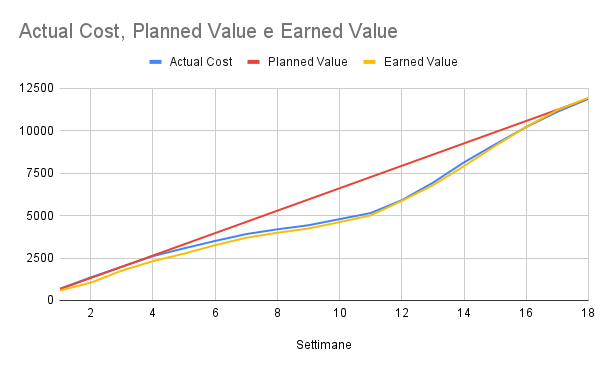
\includegraphics[scale=0.5]{AC_PV_EV.png}
\end{center}
\subsection{Cost Variance e Schedule Variance}
\begin{center}
	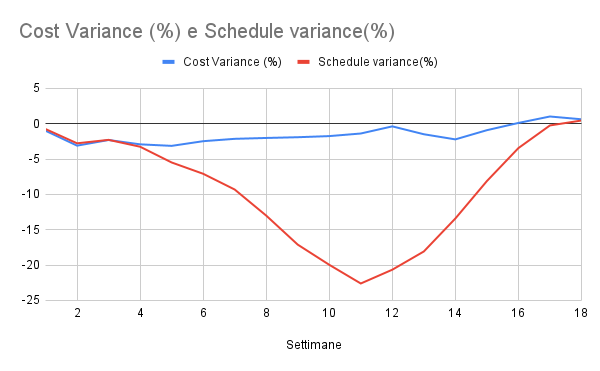
\includegraphics[scale=0.5]{Cost_Variance_Schedule_Variance.png}
\end{center}

\subsection{Eastimate at completition e Estimate to Complete}
\begin{center}
	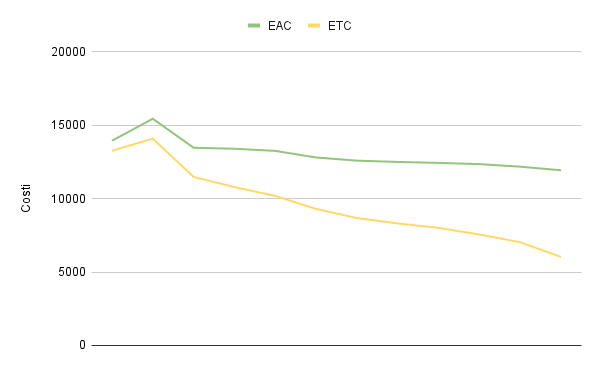
\includegraphics[scale=0.6]{EAC_ETC.png}
\end{center}
\subsection{Cost Performance Index}
\begin{center}
	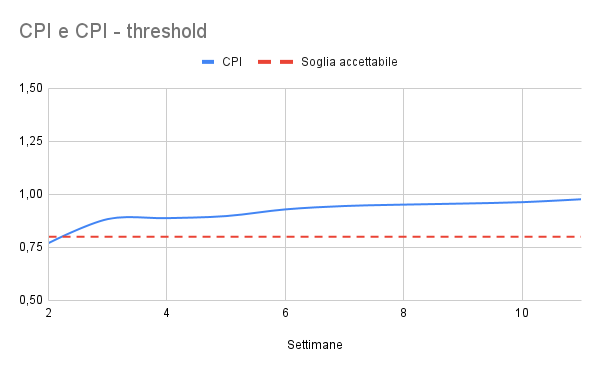
\includegraphics[scale=0.6]{CPI.png}
\end{center}
\subsection{Indice di Gulpease}
\begin{center}
	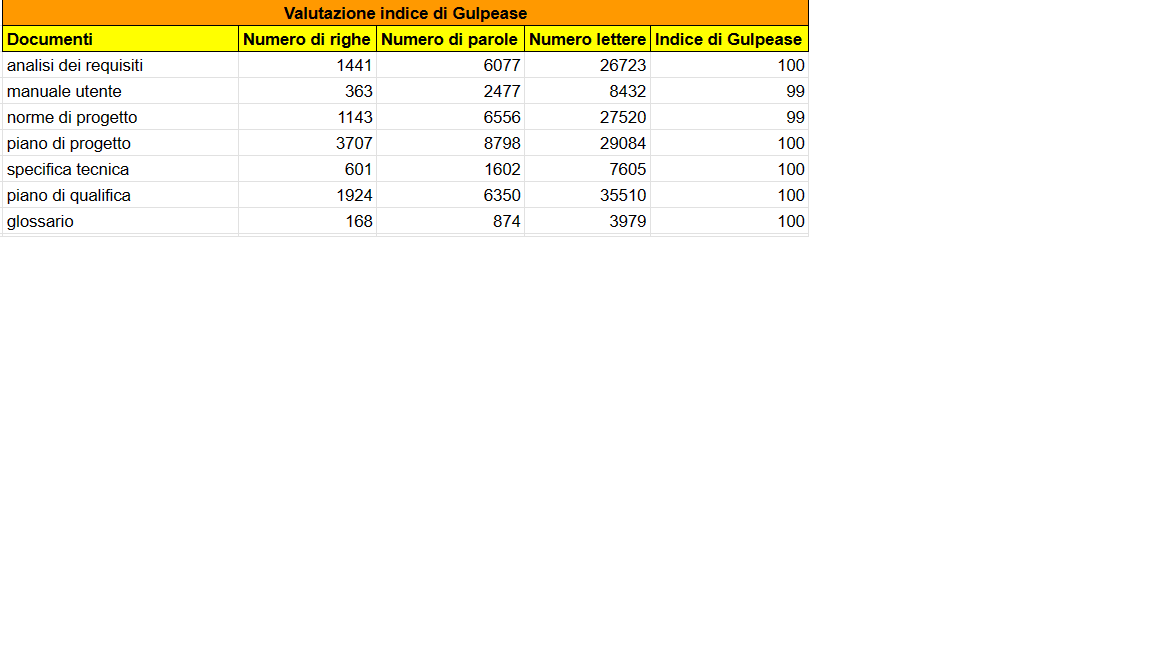
\includegraphics[scale=0.8]{Gulpease.png}
\end{center}


\subsection{Verifica del Codice}
\subsubsection{Front-end}
\begin{center}
		\begin{center}
			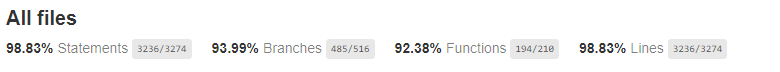
\includegraphics[scale=0.8]{totalCoverageFrontEnd.png}
		\end{center}
		L'immagine sovrastante riporta rispettivamente la Statement, Branch, Function e Code coverage \textbf{complessiva} ottenuta sulla parte di front-end del prodotto
		\begin{center}
			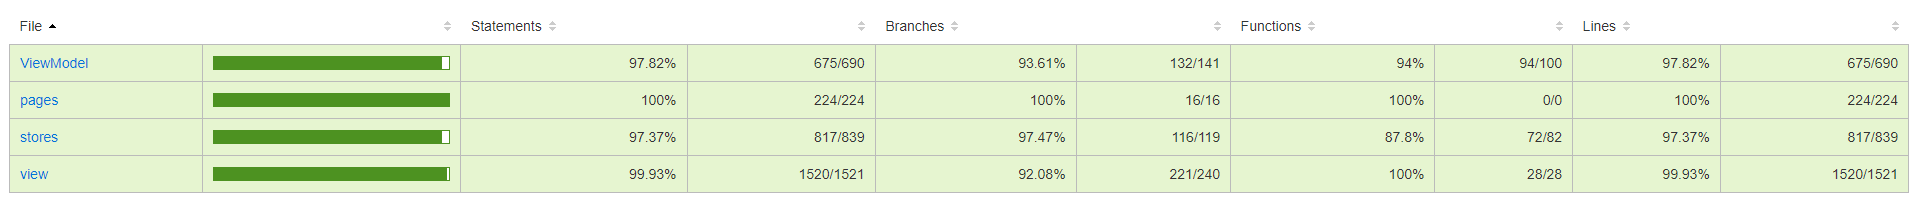
\includegraphics[scale=0.3]{test_frontEnd.png}	
		\end{center}
		L'immagine sovrastante riporta rispettivamente la Statement, Branch, Function e Code coverage ottenuta sui singoli file della parte di front-end del prodotto
\end{center}
\subsubsection{Back-end}
	\begin{center}
		
\includegraphics[scale=0.8]{totalCoverageBackEnd.png}
	\end{center}
		L'immagine sovrastante riporta rispettivamente la Statement, Branch, Function e Code coverage \textbf{complessiva} ottenuta sulla parte di back-end del prodotto
	\begin{center}
		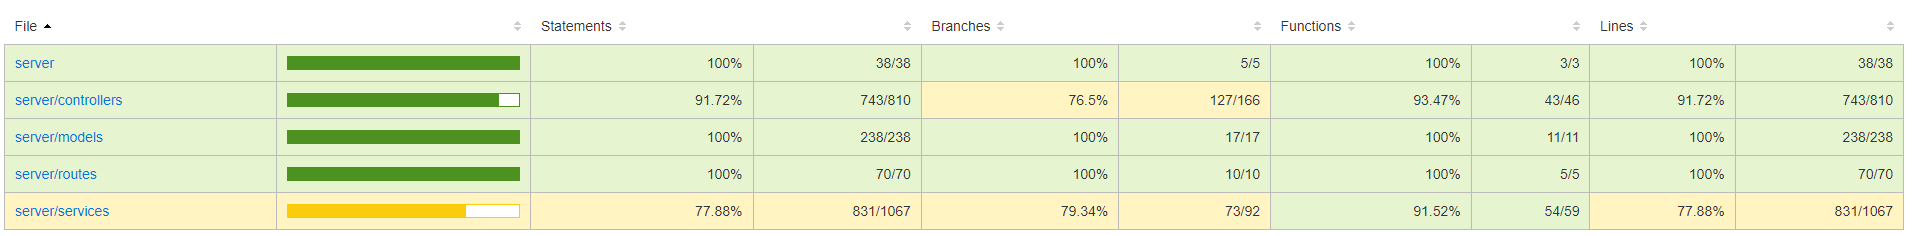
\includegraphics[scale=0.3]{test_backEnd.png}
	\end{center}
		L'immagine sovrastante riporta rispettivamente la Statement, Branch, Function e Code coverage ottenuta sui singoli file della parte di back-end del prodotto
	
\end{document}
